132. \begin{figure}[ht!]
\center{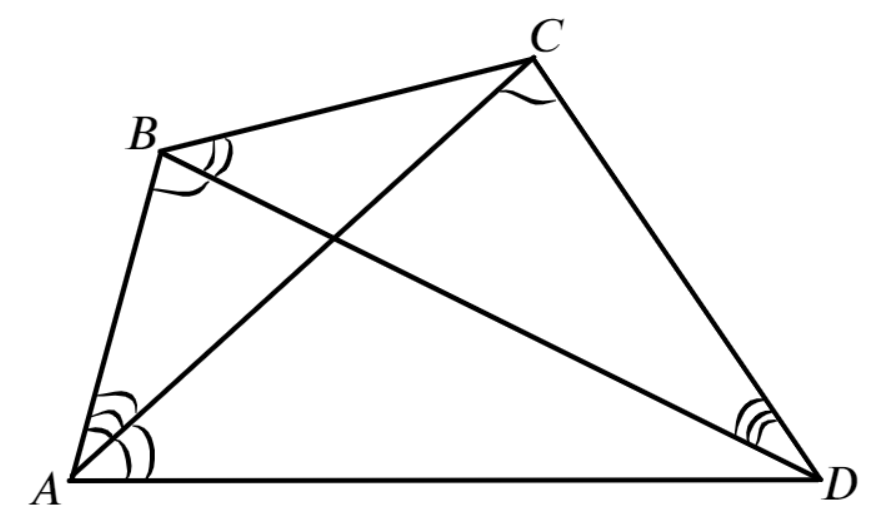
\includegraphics[scale=0.35]{g9-132.png}}
\end{figure}\\
Так как угол, образованный стороной $AB$ и диагональю $BD$ равен углу, образованному противоположной стороной $CD$ и другой диагональю $AC,$ четырёхугольник $ABCD$ является вписанным. Тогда аналогично $\angle BAC=\angle BDC,\ \angle CBD=\angle CAD,\ \angle A=\angle BAC+\angle CAD=53^\circ+64^\circ=117^\circ.$\\
